\documentclass[10pt,a4paper]{article}
\usepackage[T1]{fontenc}
\usepackage[utf8]{inputenc}
\usepackage{lmodern,textcomp}
\usepackage[a4paper,margin=22mm,headheight=14pt]{geometry}
\usepackage{amsmath,amssymb,graphicx,booktabs,array,longtable,tabularx}
\usepackage{xcolor,microtype,needspace,placeins,etoolbox}
\usepackage[numbers,sort&compress]{natbib}
\usepackage[font=small,labelfont=bf,justification=raggedright,singlelinecheck=false]{caption}
\usepackage{fancyhdr}
\usepackage[hidelinks,unicode]{hyperref}
\usepackage{lineno}
\urlstyle{same}
\definecolor{pendingcolor}{RGB}{140,80,40}
\newcommand{\pending}[1]{{\color{pendingcolor}\textnormal{[#1]}}}
\newcommand{\blankfield}[1]{\textemdash\,\textsuperscript{\pending{#1}}}
\setlength{\parindent}{0pt}
\setlength{\parskip}{5pt plus 1pt minus 1pt}
\setlength{\emergencystretch}{2em}
\setlength{\tabcolsep}{4pt}
\renewcommand{\arraystretch}{1.15}
\linespread{1.06}
\pagestyle{fancy}\fancyhf{}
\fancyhead[L]{\small MALT--SS whole-slide classification}
\fancyhead[R]{\small Research manuscript}
\fancyfoot[C]{\thepage}
\renewcommand{\headrulewidth}{0.3pt}
\renewcommand{\topfraction}{0.95}
\renewcommand{\bottomfraction}{0.95}
\renewcommand{\textfraction}{0.05}
\renewcommand{\floatpagefraction}{0.65}
\setlength{\textfloatsep}{14pt plus 2pt minus 2pt}
\makeatletter
\setlength{\@fptop}{0pt}\setlength{\@fpsep}{14pt}\setlength{\@fpbot}{0pt plus 1fil}
\makeatother

\fancyhead[R]{\small Supplementary information}
\renewcommand{\thetable}{S\arabic{table}}
\renewcommand{\thefigure}{S\arabic{figure}}
\renewcommand{\theequation}{S\arabic{equation}}
\renewcommand{\thesubsection}{S\arabic{subsection}}
\begin{document}
\begin{center}\fbox{\begin{minipage}{.92\textwidth}\small
\textbf{Public repository copy -- filtered, not the complete submission draft.}
Tissue images, individual-slide plots, case-level tables and row-level source data
are withheld. Marked omissions preserve the original numbering and captions.
References to Source Data describe the local research archive; only screened
aggregate tables are distributed here. Reported aggregate estimates are unchanged.
\end{minipage}}\end{center}\medskip
\begin{center}
{\Large\bfseries Supplementary information}\par\medskip
{\large Foundation-model-based whole-slide classification of salivary gland MALT lymphoma and Sjögren's syndrome}
\end{center}
\section*{Supplementary Methods}
% Restored from ../methods_hybrid_evidence_mil.tex and checked against
% ../../scripts/ss_experiment_suite.py: GatedAttentionPool,
% HybridEvidenceMILEncoder and SlideClassifier. This file is maintained by hand.
\subsection{Hybrid-Evidence MIL}

\paragraph{Task formulation and feature projection.}
Each WSI was represented by a sampled feature bag
$X=\{\mathbf{x}_i\}_{i=1}^{N}$ and its associated patch coordinates
$(a_i,b_i)$, where $N=512$ and $\mathbf{x}_i\in\mathbb{R}^{1536}$.
The slide label was $y=1$ for MALT and $y=0$ for SS.
No patch-level labels were used. A shared projection placed all features in a
$D=256$ dimensional hidden space:
\begin{equation}\label{eq:projection}
 \mathbf{h}_i = \operatorname{Dr}_{0.3}\!\left[
  \operatorname{GELU}\!\left(\operatorname{LN}
  (\mathbf{W}_{p}\mathbf{x}_i+\mathbf{b}_{p})\right)\right],
 \qquad \mathbf{h}_i\in\mathbb{R}^{D}.
\end{equation}
Here $\operatorname{LN}$ denotes layer normalization and $\operatorname{Dr}_{0.3}$
denotes dropout with probability 0.3 during training; dropout is disabled during
inference. All vectors below are column vectors, and $[\,\cdot\,;\,\cdot\,]$
denotes concatenation along the feature dimension.

\paragraph{Gated attention evidence.}
Gated pooling followed the attention mechanism of Ilse and colleagues
\citep{ref5}, with an additional value transformation implemented in the archived
model. For a sequence $Z=\{\mathbf{z}_j\}_{j=1}^{L}$ of $D$ dimensional vectors,
define the pooling operator $\mathcal{G}_{\theta}$ as
\begin{subequations}\label{eq:gated-pool}
\begin{align}
 \mathbf{t}_j &= \operatorname{Dr}_{0.3}
     \!\left[\operatorname{ReLU}(\mathbf{W}_{v}\mathbf{z}_j+\mathbf{b}_{v})\right],
     \label{eq:pool-value}\\
 \ell_j &= \mathbf{w}_{a}^{\mathsf T}
    \left[\tanh(\mathbf{V}\mathbf{t}_j+\mathbf{b}_{V})
     \odot\operatorname{sigmoid}(\mathbf{U}\mathbf{t}_j+\mathbf{b}_{U})\right]+b_a,
     \label{eq:pool-logit}\\
 \alpha_j &= \frac{\exp(\ell_j)}{\sum_{l=1}^{L}\exp(\ell_l)},
 \qquad \mathcal{G}_{\theta}(Z)=\sum_{j=1}^{L}\alpha_j\mathbf{t}_j.
     \label{eq:pool-sum}
\end{align}
\end{subequations}
The symbol $\odot$ denotes element-wise multiplication. All attention and value
matrices map between $D$ dimensional spaces. The attention evidence vector was
$\mathbf{e}_{\mathrm{att}}=\mathcal{G}_{\theta_A}(\{\mathbf{h}_i\}_{i=1}^{N})$.
Thus, the pooling weights multiply transformed values $\mathbf{t}_i$.
The regional branch used the same operator with independently learned parameters
$\theta_R$.

\paragraph{Distribution evidence.}
The center and heterogeneity of the sampled bag were summarized by two separate
vectors:
\begin{subequations}\label{eq:distribution}
\begin{align}
 \mathbf{e}_{\mu} &= \frac{1}{N}\sum_{i=1}^{N}\mathbf{h}_i,\\
 \mathbf{e}_{\sigma} &=
 \left[\frac{1}{N-1}\sum_{i=1}^{N}
       (\mathbf{h}_i-\mathbf{e}_{\mu})^{\odot 2}\right]^{\odot 1/2}.
\end{align}
\end{subequations}
Powers and square roots in Eq.~\eqref{eq:distribution} are element-wise. The
sample denominator $N-1$ matches the standard deviation used in the code.

\paragraph{Prototype-margin evidence.}
Two latent prototype banks indexed by $c\in\{0,1\}$ each contained
$K=8$ learnable prototypes
$\mathbf{p}_{c,r}\in\mathbb{R}^{D}$. Let a hat denote the implemented
$\ell_2$ normalization, with its numerical safeguard for zero norms.
The maximum cosine similarity within each bank and the bank-1-minus-bank-0 margin
were
\begin{subequations}\label{eq:prototype}
\begin{align}
 s_{i,c} &= \max_{1\leq r\leq K}
       \widehat{\mathbf{h}}_i^{\mathsf T}\widehat{\mathbf{p}}_{c,r},
       \qquad m_i=s_{i,1}-s_{i,0},\label{eq:margin}\\
 k &= \min(32,N),\qquad
 I_{+}=\operatorname{TopKIdx}(\{m_i\},k),\qquad
 I_{-}=\operatorname{TopKIdx}(\{-m_i\},k),\\
 \mathbf{e}_{+} &= \frac{1}{k}\sum_{i\in I_{+}}\mathbf{h}_i,
 \qquad \mathbf{e}_{-}=\frac{1}{k}\sum_{i\in I_{-}}\mathbf{h}_i.
\end{align}
\end{subequations}
$\operatorname{TopKIdx}$ returns indices of the $k$ largest entries. The high-
and low-margin vectors therefore average the instances with the largest and
smallest margins, respectively; the selected values need not all have the same
sign. Prototypes were optimized through differentiable similarity and margin
statistics in the slide-level classification objective. The hard top-$k$ index
selections were discrete; no additional prototype-specific loss or regional
labels were used. The bank indices do not identify validated MALT or SS
morphology, and a larger margin is not constrained to increase the final MALT score.

\paragraph{Coordinate-ordered groups and low-margin evidence.}
To form coordinate-ordered groups, let $\pi$ be the permutation obtained by
sorting the implemented coordinate key $10^6b_i+a_i$. The ordered hidden
sequence was partitioned using the code's chunk operation into $Q\leq16$
consecutive non-empty chunks $C_j$ (16 equal chunks for the 512 sampled patches).
Group tokens and the combined low-margin/regional vector were
\begin{subequations}\label{eq:regional}
\begin{align}
 \mathbf{r}_j &= \frac{1}{|C_j|}\sum_{l\in C_j}\mathbf{h}_{\pi(l)},
        \qquad j=1,\ldots,Q,\\
 \mathbf{e}_{\mathrm{reg}} &=
       \mathcal{G}_{\theta_R}(\{\mathbf{r}_j\}_{j=1}^{Q}),
       \qquad \mathbf{e}_{\mathrm{nr}}=\mathbf{e}_{-}+\mathbf{e}_{\mathrm{reg}}.
\end{align}
\end{subequations}
The regional operator includes its own value transformation from
Eq.~\eqref{eq:pool-value}. Coordinates determine group membership, but the
subsequent pooling is invariant to the order of the group tokens. The branch
has no explicit intergroup distances, adjacency or positional encoding.
Equal-sized groups of sampled instances were not anatomical regions and can
span different physical extents.

\paragraph{Similarity and margin statistics.}
Eight scalar statistics supplemented the evidence vectors. Define
$T_c=\operatorname{TopKIdx}(\{s_{i,c}\},k)$,
$\bar{s}_{c}^{\mathrm{top}}=k^{-1}\sum_{i\in T_c}s_{i,c}$ and
$\bar{m}=N^{-1}\sum_i m_i$. Then
\begin{subequations}\label{eq:statistics}
\begin{align}
 s_m &= \left[\frac{1}{N-1}\sum_{i=1}^{N}(m_i-\bar m)^2\right]^{1/2},\\
 \rho_0 &= \frac{1}{N}\sum_{i=1}^{N}\mathbb{I}(m_i>0),\qquad
 \rho_{\bar m}=\frac{1}{N}\sum_{i=1}^{N}\mathbb{I}(m_i>\bar m),\\
 \mathbf{u} &= \bigl[\bar{s}_{0}^{\mathrm{top}},\bar{s}_{1}^{\mathrm{top}},
       \bar m,s_m,\max_i m_i,\min_i m_i,\rho_0,\rho_{\bar m}\bigr]^{\mathsf T}
       \in\mathbb{R}^{8}.
\end{align}
\end{subequations}
$\mathbb{I}$ is the indicator function. The top-similarity sets $T_c$ are computed
separately for the two banks and need not coincide with the margin-based sets
$I_{+}$ and $I_{-}$.

\paragraph{Learned gating, weighted concatenation and classification.}
The five evidence vectors were ordered as
$(\mathbf{e}_1,\ldots,\mathbf{e}_5)=
(\mathbf{e}_{\mathrm{att}},\mathbf{e}_{\mu},\mathbf{e}_{\sigma},
 \mathbf{e}_{+},\mathbf{e}_{\mathrm{nr}})$.
A two-layer gate received the unweighted vectors and statistics:
\begin{subequations}\label{eq:fusion}
\begin{align}
 \mathbf{q} &= [\mathbf{e}_1;\mathbf{e}_2;\mathbf{e}_3;\mathbf{e}_4;
                   \mathbf{e}_5;\mathbf{u}]\in\mathbb{R}^{5D+8},\\
 \boldsymbol{\gamma} &= \operatorname{softmax}\!\left(
    \mathbf{W}_{g2}\operatorname{Dr}_{0.3}\!\left[
       \operatorname{GELU}(\mathbf{W}_{g1}\mathbf{q}+\mathbf{b}_{g1})\right]
       +\mathbf{b}_{g2}\right)\in\mathbb{R}^{5},\label{eq:gate}\\
 \widetilde{\mathbf{q}} &= [\gamma_1\mathbf{e}_1;\gamma_2\mathbf{e}_2;
       \gamma_3\mathbf{e}_3;\gamma_4\mathbf{e}_4;\gamma_5\mathbf{e}_5;
       \mathbf{u}],\label{eq:weighted-concat}\\
 \mathbf{z} &= \operatorname{Dr}_{0.3}\!\left[
       \operatorname{GELU}\!\left(\operatorname{LN}
       (\mathbf{W}_{f}\widetilde{\mathbf{q}}+\mathbf{b}_{f})\right)\right],\\
 a &= \mathbf{w}_{o}^{\mathsf T}\operatorname{Dr}_{0.3}\!\left[
       \operatorname{ReLU}\!\left(\operatorname{LN}
       (\mathbf{W}_{c}\mathbf{z}+\mathbf{b}_{c})\right)\right]+b_o,
       \qquad p=\operatorname{sigmoid}(a).
\end{align}
\end{subequations}
The gate dimensions were $\mathbf{W}_{g1}\in\mathbb{R}^{D\times(5D+8)}$
and $\mathbf{W}_{g2}\in\mathbb{R}^{5\times D}$;
$\mathbf{W}_{f}\in\mathbb{R}^{D\times(5D+8)}$ and
$\mathbf{W}_{c}\in\mathbb{R}^{D\times D}$.
Each $\gamma_j$ is non-negative and $\sum_j\gamma_j=1$.
Equation~\eqref{eq:weighted-concat} preserves five weighted feature blocks;
the eight statistics enter fusion without multiplication by a branch weight.
The gate supplies sample-dependent feature scaling, rather than a distribution
of causal contributions. Branch norms, the learned fusion transformation and
the ungated statistics also affect the classifier. The output $p$ is an
uncalibrated MALT model score in $[0,1]$.

\paragraph{Training objective.}
For a minibatch $\mathcal{B}$ of slides, the weighted binary cross-entropy was
\begin{equation}\label{eq:loss}
 \mathcal{L}=-\frac{1}{|\mathcal{B}|}\sum_{b\in\mathcal{B}}
 \left[w_{+}y_b\log p_b+(1-y_b)\log(1-p_b)\right],
 \qquad w_{+}=\frac{77}{67}.
\end{equation}
The implementation evaluated this objective directly from logits for numerical
stability. The positive-class weight was the ratio of the 77 SS to 67 MALT
training slides. Class weighting changes the optimum of binary cross-entropy;
the sigmoid output was not assumed to equal an unweighted posterior probability.
No calibration model was fitted to either evaluation set. Optimization and the
archived checkpoint are described below.

\subsection{Historical model settings and exploratory ensembles}
The retained Hybrid checkpoint contains 1,521,672 parameters and was selected at epoch 15 from a 30-epoch run with batch size eight. The archived ABMIL contains 6,690,306 parameters, retains a 1,536-dimensional representation and was selected at epoch 37 from a 50-epoch run with batch size 16. Both use learning rate $5\times10^{-5}$ and weight decay $10^{-4}$. The classifier and attention dimensions differ; these comparisons evaluate complete implementations. The checkpoint inventory in Source Data supplies exact dimensions, training budgets and identities for the inspected models.

The local CLAM-style implementation omits the original instance-clustering loss. The local two-tier attention model uses partitioned bags and two aggregation stages; the transformer variant uses a conventional transformer and coordinate multilayer perceptron. The grouped-region transformer averages coordinate-ordered groups before transformer processing. The latter is not the published R$^2$T feature re-embedding architecture \citep{rrt2024}. Prototype-pooling names describe local implementations and are not assigned an unsupported correspondence to a specific published ProtoMIL method. Table~S1 retains all historical results under these descriptive names; the code-ID mapping accompanies the data.

The historical ensemble was explored by enumerating combinations of candidate predictions and ranking them by internal AUROC and AP. Hybrid, local CLAM-style pooling and the grouped-region transformer were combined by equal probability averaging. Its internal AUROC was 0.9649. At threshold 0.5 it had 21 true positives, 22 true negatives, four false positives and two false negatives. The separately explored threshold 0.70 yielded 21, 25, one and two, respectively, and accuracy 93.88\%. Both member selection and threshold exploration used development outputs; this is not a prespecified independent validation result. The historical three-model ensemble was not evaluated externally.

Earlier compound configurations and seed experiments are preserved in the historical Source Data. Enabling the high-margin vector also enabled eight statistics, and low-margin/regional components were added together. Moreover, training patch samples used an unseeded NumPy generator in that component study. Its results cannot independently attribute performance to each module. Earlier seeds 7, 13 and 21 used 20 epochs, whereas seed 42 used 30, with differing partitions. They are not pooled with the later controlled seeds.

\subsection{Controlled training and algorithm screen}
The first matched experiment used attention-only, full fixed scaling and full learned gating, each with seeds 17, 29 and 43. Attention-only retained the shared projection and attention/classifier dimensions; fixed scaling multiplied each of the five vectors by 0.2 while retaining the statistics and fusion layer. Their parameter counts were 658,178, 1,190,403 and 1,521,672. Within each seed, shared tensors were identically initialized. Exact training bags and minibatch orders were matched, but masks after divergent computation branches were not assumed to be elementwise identical.

The later screen trained ten configurations with the same three seeds (30 runs), then the chosen candidate and Hybrid with seeds 59 and 71 (four runs). The attention and Hybrid controls reproduced the first matched experiment's selected epochs and classifications, with maximum score discrepancy $5.96\times10^{-8}$. Thus, the studies include nine prior runs and 34 later runs, with six deliberately repeated controls, not 43 independent initialization settings.

Common settings were 30 epochs, AdamW with learning rate $5\times10^{-5}$, weight decay $10^{-4}$, batch size eight, positive loss weight $77/67$ and dropout 0.3. The first strictly highest validation-AUROC epoch was retained. There was no scheduler, early stopping, probability calibration or threshold optimization. The following deviations define the screen:
\begin{itemize}
\item \textbf{Input L2 normalization:} each 1,536-dimensional patch vector was divided by its norm (safeguard $10^{-12}$) and multiplied by $\sqrt{1536}$ before Hybrid or matched attention. This changes input magnitude as well as removing norm variation.
\item \textbf{Attention masking:} six randomly chosen logits among the top ten attention logits were masked during training. Evaluation used unmasked attention. This is an STKIM-inspired component adaptation, not full ACMIL \citep{acmil2024}.
\item \textbf{Original-space attention:} gated attention with hidden dimension 256 pooled the original 1,536-dimensional values, followed by a linear classifier; dropout was 0.25.
\item \textbf{Feature-subspace attention:} a shared sorted random subset of 256 feature coordinates was used for attention within each training minibatch, while values retained all 1,536 dimensions. At inference, logits from 21 contiguous 256-coordinate windows with stride 64 were averaged before sigmoid. A separate configuration used batch size 32 and learning rate $3\times10^{-4}$, changing both optimization factors and the update count (150 versus 540). These are nnMIL-inspired adaptations under the local 30-epoch protocol \citep{nnmil2026}.
\item \textbf{Two-bag training:} classification losses from two independently sampled 512-patch bags were averaged. The consistency variant added 0.1 times symmetric Bernoulli KL divergence. For logits $z_1,z_2$, this was implemented as $\tfrac12\operatorname{mean}[(\sigma(z_1)-\sigma(z_2))(z_1-z_2)]$, with gradients through both paths. Patch samples and dropout both varied; this extends the perturbation beyond original R-Drop \citep{rdrop2021}. The two-bag classifier without KL was the corresponding control.
\end{itemize}

The eight modified candidates were ranked by mean validation AUROC over seeds 17, 29 and 43, rounded to 12 decimal places. Ties used smaller sample SD, then parameter count and configuration ID. The selected Attention+L2 configuration was frozen before further seed training and new external inference. The predefined engineering target was an internal mean AUROC increase of at least 0.01 over Hybrid, with at least two non-decreasing paired seeds; a mean balanced-accuracy drop exceeding 0.02 was flagged. The observed increase was 0.0011, so the target was not met. Added seeds and external results did not trigger reselection. All 34 runs are in Table~S5; the complete protocol is included with the source bundle.

Raw-mean and normalized-mean logistic controls were fitted to full-feature slide means from the training set. Training-only standardization and fixed logistic hyperparameters prevented evaluation slides from contributing to fitted feature scaling. Their 512-patch and full-feature inference results are separate. The former uses the common reference bags, whereas the latter uses every available feature row (Table~S6).

\subsection{Sampling rules, reproducibility and statistics}
Training bag seeds were derived from the first four SHA-256 bytes, interpreted as an unsigned little-endian 32-bit integer. Shared controlled-run seeds encoded the training seed, epoch and slide code; order and dropout used separate keys. Two-view training used a distinct second-view key. Exact indices and orders were archived. The original reference evaluation retained full external-manifest indices even after the final subset was selected. For historical fixed-checkpoint resampling, 20 new per-slide bags used keys encoding study date, cohort, publication-coded slide and repeat. Sampling was without replacement unless fewer than 512 rows existed; historical internal indices were sorted when sampling without replacement. The later five-bag study used a distinct fixed key, so those five bags exclude the reference bag.

Probability ensembles averaged every specified seed and bag; no seed was omitted. The subspace model's within-model feature-window \emph{logit} averaging is distinct from between-model probability averaging. Bootstrap comparisons used aligned resamples across models. The paired external difference for five-seed/five-bag Attention+L2 minus Hybrid was $-0.0164$ (95\% interval $-0.0448$ to 0.0058). Its difference from the historical primary checkpoint was $-0.0407$ ($-0.1320$ to 0.0267); these are different comparators, not interchangeable baselines. All intervals are conditional on the saved predictions.

Primary Hybrid, ABMIL and other reference predictions were reproduced before the comparative analyses. An independent CPU audit of the later screen verified all 8,246 main prediction rows and 76 metric rows, and checked six predictions per neural checkpoint (204 in total; maximum CPU/GPU discrepancy $1.79\times10^{-7}$). Sampling indices, train-only linear standardization and ensemble calculations were independently checked. These are numerical-reproducibility checks, not additional clinical validation.

The analyses used Python 3.10.18, NumPy 1.26.4, pandas 2.3.2, SciPy 1.15.3, scikit-learn 1.7.2 and Matplotlib 3.10.6. Later inference/training used PyTorch 2.8.0 and CUDA 12.8 on an NVIDIA A800 80GB. The 34-run algorithm workflow, including loading and evaluation, took 620.9 seconds and peaked at 4.70GiB of PyTorch-allocated GPU memory; it reused cached features. This is a local shared-hardware observation, not an independently benchmarked runtime. The historical training runtime remains completion item T02.

\subsection{Acquisition and image-region audit}
Header-derived scan software was NDP.scan 2.5.85 for 133 internal slides and 3.3.0 for 60; all 168 analyzed external slides recorded 2.5.85. Extraction attributes recorded zero overlap and a 1,024-pixel level-0 patch footprint. These acquisition fields do not determine clinical provenance or actual stain. The inspected TRIDENT checkout identifies version 0.2.0 and revision prefix a6305acfef68. Full local file identities are retained in the project provenance record; the exact encoder-weight revision remains T01.

The four illustrated model cases comprise a MALT true positive, SS true negative, SS false positive and MALT false negative. Across 12 visualization cases, the largest absolute performance--visualization score difference was 0.3252, without a threshold classification change. Margin colors were normalized independently per slide using a symmetric scale based on the 2nd and 98th percentiles, so color intensity is not directly comparable across slides. The mean-feature gate was the largest on all 217 reference bags; a gate is a feature-scaling coefficient, not a contribution decomposition.

All eight displayed thumbnails matched their original 1,024-pixel windows after the archived resize to 220 pixels. The corresponding field width was approximately 231.1$\,\mu$m, supporting 50-$\mu$m bars. Automated segmentation coverage was 100\% for seven windows and 48.11\% for the low-margin window in the false-negative case. Polygon holes were included by the archived segmentation convention, so these are geometric mask overlaps, not verified tissue fractions. For that case, archived overlay geometry used a slide height of 62,208 pixels, whereas the current reader reported 70,400; the original geometry is preserved. Its near-empty-looking crop has not been replaced or interpreted as a mechanism of failure. Pathology review and geometry resolution remain completion item H06. The separate illustrative photomicrographs lack original physical calibration and are labeled accordingly.

\clearpage
\section*{Supplementary Tables}
{\small\begin{longtable}{>{\raggedright\arraybackslash}p{0.44\textwidth}>{\raggedright\arraybackslash}p{0.1\textwidth}>{\raggedright\arraybackslash}p{0.1\textwidth}>{\raggedright\arraybackslash}p{0.12\textwidth}>{\raggedright\arraybackslash}p{0.12\textwidth}}
\caption{Historical complete-implementation comparison on 49 validation slides}\\
\toprule
\textbf{Implementation} & \textbf{AUROC} & \textbf{AP} & \textbf{Sens. (\%)} & \textbf{Spec. (\%)} \\
\midrule\endfirsthead
\toprule
\textbf{Implementation} & \textbf{AUROC} & \textbf{AP} & \textbf{Sens. (\%)} & \textbf{Spec. (\%)} \\
\midrule\endhead
Three-model ensemble & 0.9649 & 0.9576 & 91.30 & 84.62 \\
Hybrid & 0.9599 & 0.9514 & 95.65 & 80.77 \\
ABMIL & 0.9498 & 0.9396 & 82.61 & 88.46 \\
Local two-tier attention & 0.9398 & 0.9416 & 86.96 & 88.46 \\
Local attention pooling (CLAM-style) & 0.9365 & 0.9422 & 91.30 & 84.62 \\
Local grouped-region transformer & 0.9281 & 0.8400 & 95.65 & 84.62 \\
Local prototype pooling & 0.9264 & 0.9306 & 86.96 & 84.62 \\
Mean pooling & 0.9247 & 0.9332 & 78.26 & 92.31 \\
Local transformer pooling & 0.9231 & 0.9180 & 65.22 & 96.15 \\
Local dual-stream pooling & 0.9197 & 0.9260 & 78.26 & 92.31 \\
Distribution--prototype pooling & 0.9130 & 0.9178 & 91.30 & 69.23 \\
CONCH v1.5 + TITAN & 0.9013 & 0.9203 & 91.30 & 73.08 \\
\bottomrule\end{longtable}}
{\footnotesize Threshold 0.5. This table retains all historical models, not a ranking of official full-method reproductions. TITAN uses a different encoder and instance budget. Code-ID mappings and original metrics are in Source Data. The ensemble combines Hybrid, local CLAM-style pooling and the grouped-region transformer.}

{\small\begin{longtable}{>{\raggedright\arraybackslash}p{0.39\textwidth}>{\raggedright\arraybackslash}p{0.11\textwidth}>{\raggedright\arraybackslash}p{0.13\textwidth}>{\raggedright\arraybackslash}p{0.13\textwidth}>{\raggedright\arraybackslash}p{0.15\textwidth}}
\caption{External complete-checkpoint comparison on identical reference bags}\\
\toprule
\textbf{Implementation} & \textbf{AUROC} & \textbf{Sens. (\%)} & \textbf{Spec. (\%)} & \textbf{TP/FN/\allowbreak TN/FP} \\
\midrule\endfirsthead
\toprule
\textbf{Implementation} & \textbf{AUROC} & \textbf{Sens. (\%)} & \textbf{Spec. (\%)} & \textbf{TP/FN/\allowbreak TN/FP} \\
\midrule\endhead
Hybrid & 0.8721 & 93.42 & 68.75 & 142/10/11/5 \\
ABMIL & 0.7903 & 42.76 & 81.25 & 65/87/13/3 \\
Local attention pooling (CLAM-style) & 0.6591 & 58.55 & 62.50 & 89/63/10/6 \\
Local grouped-region transformer & 0.7743 & 89.47 & 50.00 & 136/16/8/8 \\
\bottomrule\end{longtable}}

{\small\begin{longtable}{>{\raggedright\arraybackslash}p{0.27\textwidth}>{\raggedright\arraybackslash}p{0.17\textwidth}>{\raggedright\arraybackslash}p{0.23\textwidth}>{\raggedright\arraybackslash}p{0.23\textwidth}}
\caption{Three-seed controlled training comparison}\\
\toprule
\textbf{Configuration} & \textbf{Parameters} & \textbf{Validation AUROC} & \textbf{External AUROC} \\
\midrule\endfirsthead
\toprule
\textbf{Configuration} & \textbf{Parameters} & \textbf{Validation AUROC} & \textbf{External AUROC} \\
\midrule\endhead
Matched attention & 658178 & 0.9348 $\pm$ 0.0044 & 0.7270 $\pm$ 0.1035 \\
Full fixed scaling & 1190403 & 0.9398 $\pm$ 0.0153 & 0.7445 $\pm$ 0.1254 \\
Full learned gate & 1521672 & 0.9353 $\pm$ 0.0070 & 0.7633 $\pm$ 0.1581 \\
\bottomrule\end{longtable}}
{\footnotesize Seeds 17, 29 and 43. Means $\pm$ sample SD. The algorithm screen reran the attention and learned-gate controls and reproduced them; those reruns are not new independent seeds.}

{\small\begin{longtable}{>{\raggedright\arraybackslash}p{0.43\textwidth}>{\raggedright\arraybackslash}p{0.23\textwidth}>{\raggedright\arraybackslash}p{0.23\textwidth}}
\caption{All ten configurations in the three-seed algorithm screen}\\
\toprule
\textbf{Configuration} & \textbf{Validation AUROC} & \textbf{External AUROC} \\
\midrule\endfirsthead
\toprule
\textbf{Configuration} & \textbf{Validation AUROC} & \textbf{External AUROC} \\
\midrule\endhead
Hybrid control & 0.9353 $\pm$ 0.0070 & 0.7633 $\pm$ 0.1581 \\
Matched attention & 0.9348 $\pm$ 0.0044 & 0.7270 $\pm$ 0.1035 \\
Hybrid + L2 & 0.9337 $\pm$ 0.0140 & 0.7166 $\pm$ 0.2016 \\
Attention + L2 & 0.9365 $\pm$ 0.0060 & 0.7726 $\pm$ 0.1111 \\
Attention masking & 0.9348 $\pm$ 0.0073 & 0.7356 $\pm$ 0.0940 \\
Original-space attention & 0.9041 $\pm$ 0.0463 & 0.6051 $\pm$ 0.2023 \\
Feature-subspace attention & 0.8701 $\pm$ 0.0174 & 0.7876 $\pm$ 0.0617 \\
Subspace, batch32/lr3e-4 & 0.8790 $\pm$ 0.0070 & 0.7707 $\pm$ 0.0504 \\
Hybrid, two bags & 0.9337 $\pm$ 0.0245 & 0.6886 $\pm$ 0.2175 \\
Hybrid, two bags + KL & 0.9337 $\pm$ 0.0235 & 0.7307 $\pm$ 0.1694 \\
\bottomrule\end{longtable}}

{\small\begin{longtable}{>{\raggedright\arraybackslash}p{0.31\textwidth}>{\raggedright\arraybackslash}p{0.06\textwidth}>{\raggedright\arraybackslash}p{0.07\textwidth}>{\raggedright\arraybackslash}p{0.1\textwidth}>{\raggedright\arraybackslash}p{0.1\textwidth}>{\raggedright\arraybackslash}p{0.11\textwidth}>{\raggedright\arraybackslash}p{0.11\textwidth}}
\caption{All 34 neural training runs: selected checkpoint results}\\
\toprule
\textbf{Configuration} & \textbf{Seed} & \textbf{Epoch} & \textbf{Val. AUC} & \textbf{Ext. AUC} & \textbf{Ext. sens.} & \textbf{Ext. spec.} \\
\midrule\endfirsthead
\toprule
\textbf{Configuration} & \textbf{Seed} & \textbf{Epoch} & \textbf{Val. AUC} & \textbf{Ext. AUC} & \textbf{Ext. sens.} & \textbf{Ext. spec.} \\
\midrule\endhead
Hybrid control & 17 & 29 & 0.9298 & 0.7311 & 60.53 & 68.75 \\
Matched attention & 17 & 13 & 0.9314 & 0.8170 & 80.26 & 62.50 \\
Hybrid + L2 & 17 & 26 & 0.9264 & 0.6571 & 74.34 & 56.25 \\
Attention + L2 & 17 & 19 & 0.9314 & 0.8976 & 73.03 & 93.75 \\
Attention masking & 17 & 13 & 0.9314 & 0.8100 & 75.00 & 62.50 \\
Original-space attention & 17 & 30 & 0.8980 & 0.5391 & 52.63 & 50.00 \\
Feature-subspace attention & 17 & 29 & 0.8562 & 0.7788 & 50.00 & 75.00 \\
Subspace, batch32/lr3e-4 & 17 & 28 & 0.8813 & 0.7722 & 54.61 & 75.00 \\
Hybrid, two bags & 17 & 8 & 0.9114 & 0.6525 & 62.50 & 56.25 \\
Hybrid, two bags + KL & 17 & 8 & 0.9114 & 0.6727 & 59.21 & 56.25 \\
Hybrid control & 29 & 20 & 0.9331 & 0.9350 & 59.21 & 93.75 \\
Matched attention & 29 & 18 & 0.9331 & 0.7500 & 61.18 & 62.50 \\
Hybrid + L2 & 29 & 18 & 0.9247 & 0.9412 & 65.79 & 93.75 \\
Attention + L2 & 29 & 18 & 0.9348 & 0.7352 & 60.53 & 62.50 \\
Attention masking & 29 & 18 & 0.9298 & 0.7669 & 51.97 & 68.75 \\
Original-space attention & 29 & 26 & 0.9532 & 0.4441 & 28.95 & 50.00 \\
Feature-subspace attention & 29 & 11 & 0.8896 & 0.7307 & 78.95 & 50.00 \\
Subspace, batch32/lr3e-4 & 29 & 4 & 0.8846 & 0.7196 & 78.95 & 37.50 \\
Hybrid, two bags & 29 & 15 & 0.9298 & 0.9219 & 83.55 & 87.50 \\
Hybrid, two bags + KL & 29 & 10 & 0.9314 & 0.9215 & 71.71 & 93.75 \\
Hybrid control & 43 & 29 & 0.9431 & 0.6238 & 17.76 & 68.75 \\
Matched attention & 43 & 12 & 0.9398 & 0.6139 & 34.87 & 56.25 \\
Hybrid + L2 & 43 & 26 & 0.9498 & 0.5514 & 22.37 & 56.25 \\
Attention + L2 & 43 & 21 & 0.9431 & 0.6850 & 45.39 & 62.50 \\
Attention masking & 43 & 22 & 0.9431 & 0.6299 & 61.18 & 56.25 \\
Original-space attention & 43 & 2 & 0.8612 & 0.8322 & 95.39 & 43.75 \\
Feature-subspace attention & 43 & 7 & 0.8645 & 0.8532 & 88.16 & 56.25 \\
Subspace, batch32/lr3e-4 & 43 & 30 & 0.8712 & 0.8203 & 63.82 & 68.75 \\
Hybrid, two bags & 43 & 12 & 0.9599 & 0.4914 & 21.71 & 50.00 \\
Hybrid, two bags + KL & 43 & 28 & 0.9582 & 0.5979 & 20.39 & 68.75 \\
Hybrid control & 59 & 20 & 0.9515 & 0.8236 & 44.08 & 87.50 \\
Attention + L2 & 59 & 22 & 0.9214 & 0.8409 & 48.68 & 93.75 \\
Hybrid control & 71 & 27 & 0.9164 & 0.9145 & 64.47 & 93.75 \\
Attention + L2 & 71 & 24 & 0.9398 & 0.8717 & 50.66 & 93.75 \\
\bottomrule\end{longtable}}
{\footnotesize Sensitivities and specificities are percentages at threshold 0.5. Every planned run is retained. Full epoch histories and checkpoints remain in the experiment archive.}

{\small\begin{longtable}{>{\raggedright\arraybackslash}p{0.15\textwidth}>{\raggedright\arraybackslash}p{0.18\textwidth}>{\raggedright\arraybackslash}p{0.14\textwidth}>{\raggedright\arraybackslash}p{0.11\textwidth}>{\raggedright\arraybackslash}p{0.14\textwidth}>{\raggedright\arraybackslash}p{0.14\textwidth}}
\caption{Deterministic linear controls}\\
\toprule
\textbf{Features} & \textbf{Input} & \textbf{Cohort} & \textbf{AUROC} & \textbf{Sens. (\%)} & \textbf{Spec. (\%)} \\
\midrule\endfirsthead
\toprule
\textbf{Features} & \textbf{Input} & \textbf{Cohort} & \textbf{AUROC} & \textbf{Sens. (\%)} & \textbf{Spec. (\%)} \\
\midrule\endhead
Raw mean & 512 patches & internal & 0.9314 & 78.26 & 92.31 \\
Raw mean & Full features & internal & 0.9264 & 78.26 & 92.31 \\
L2 mean & 512 patches & internal & 0.9247 & 73.91 & 92.31 \\
L2 mean & Full features & internal & 0.9247 & 73.91 & 92.31 \\
Raw mean & 512 patches & external & 0.8335 & 45.39 & 93.75 \\
Raw mean & Full features & external & 0.8396 & 45.39 & 93.75 \\
L2 mean & 512 patches & external & 0.8462 & 46.05 & 93.75 \\
L2 mean & Full features & external & 0.8475 & 44.74 & 93.75 \\
\bottomrule\end{longtable}}

{\small\begin{longtable}{>{\raggedright\arraybackslash}p{0.2\textwidth}>{\raggedright\arraybackslash}p{0.24\textwidth}>{\raggedright\arraybackslash}p{0.13\textwidth}>{\raggedright\arraybackslash}p{0.1\textwidth}>{\raggedright\arraybackslash}p{0.11\textwidth}>{\raggedright\arraybackslash}p{0.11\textwidth}}
\caption{Probability ensembles of the complete seed sets}\\
\toprule
\textbf{Model} & \textbf{Averaging} & \textbf{Cohort} & \textbf{AUROC} & \textbf{Sens. (\%)} & \textbf{Spec. (\%)} \\
\midrule\endfirsthead
\toprule
\textbf{Model} & \textbf{Averaging} & \textbf{Cohort} & \textbf{AUROC} & \textbf{Sens. (\%)} & \textbf{Spec. (\%)} \\
\midrule\endhead
Attention + L2 & 3 seeds; ref. bag & external & 0.7817 & 55.26 & 68.75 \\
Attention + L2 & 3 seeds; ref. bag & internal & 0.9431 & 82.61 & 88.46 \\
Hybrid control & 3 seeds; ref. bag & external & 0.7730 & 40.13 & 81.25 \\
Hybrid control & 3 seeds; ref. bag & internal & 0.9482 & 91.30 & 88.46 \\
Attention + L2 & 5 seeds; ref. bag & external & 0.8199 & 53.29 & 81.25 \\
Attention + L2 & 5 seeds; ref. bag & internal & 0.9365 & 82.61 & 92.31 \\
Hybrid control & 5 seeds; ref. bag & external & 0.8470 & 47.37 & 93.75 \\
Hybrid control & 5 seeds; ref. bag & internal & 0.9515 & 91.30 & 92.31 \\
Attention + L2 & 5 seeds; 5 bags & external & 0.8314 & 53.95 & 87.50 \\
Attention + L2 & 5 seeds; 5 bags & internal & 0.9381 & 91.30 & 88.46 \\
Hybrid control & 5 seeds; 5 bags & external & 0.8479 & 48.03 & 93.75 \\
Hybrid control & 5 seeds; 5 bags & internal & 0.9548 & 91.30 & 92.31 \\
\bottomrule\end{longtable}}
{\footnotesize Reference bags and the five newly sampled bags are separate inputs. Each displayed metric is calculated after probability averaging; it is not an average of AUROCs.}

{\small\begin{longtable}{>{\raggedright\arraybackslash}p{0.13\textwidth}>{\raggedright\arraybackslash}p{0.18\textwidth}>{\raggedright\arraybackslash}p{0.17\textwidth}>{\raggedright\arraybackslash}p{0.24\textwidth}>{\raggedright\arraybackslash}p{0.17\textwidth}}
\caption{Twenty-bag sensitivity analysis of the retained Hybrid checkpoint}\\
\toprule
\textbf{Cohort} & \textbf{Median score SD} & \textbf{Crossing 0.5} & \textbf{Draw AUROC range} & \textbf{Mean-score AUROC} \\
\midrule\endfirsthead
\toprule
\textbf{Cohort} & \textbf{Median score SD} & \textbf{Crossing 0.5} & \textbf{Draw AUROC range} & \textbf{Mean-score AUROC} \\
\midrule\endhead
internal & 0.0120 & 7/49 & 0.9498--0.9682 & 0.9632 \\
external & 0.0150 & 18/168 & 0.8549--0.8943 & 0.8775 \\
\bottomrule\end{longtable}}

\begin{table}[htbp]\centering
\caption{Linked performance and visualization outputs}
\small Individual-case rows are omitted from this public repository copy.
\end{table}

\clearpage
\begin{figure}[p]\centering
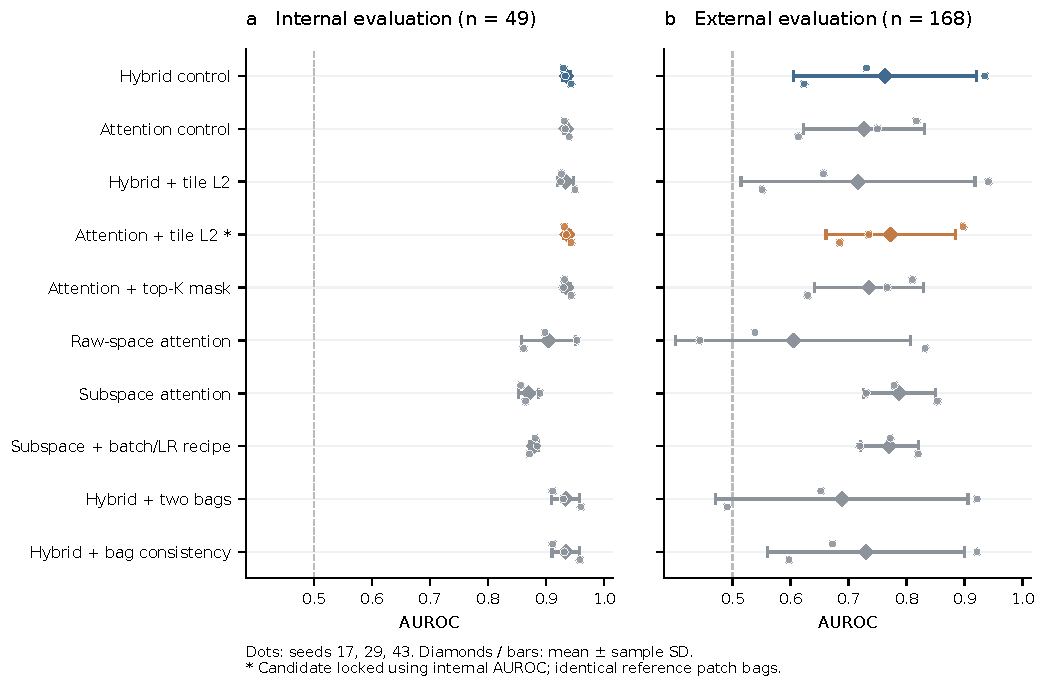
\includegraphics[width=\textwidth,height=.73\textheight,keepaspectratio]{figures/Figure_A1_all_configurations.pdf}
\caption{\textbf{Complete algorithm screen.} All ten configurations and all initial seeds (17, 29, 43) are shown for validation and external evaluation. Individual points are separately trained models; bars summarize mean and sample SD, not confidence intervals. Attention+L2 was selected on mean validation AUROC before external inference. Each cohort contains the same 49 or 168 slides across configurations.}
\end{figure}
\begin{figure}[p]\centering
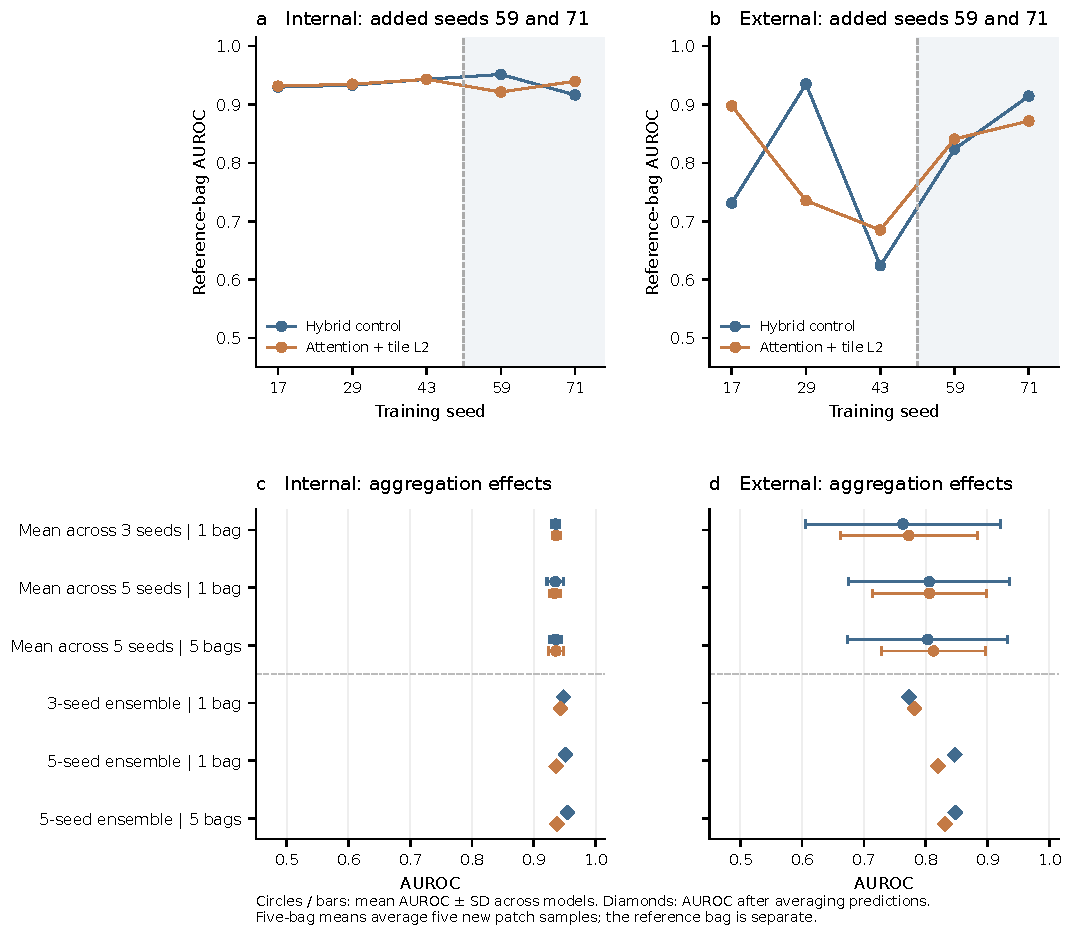
\includegraphics[width=\textwidth,height=.73\textheight,keepaspectratio]{figures/Figure_A2_stability_and_aggregation.pdf}
\caption{\textbf{Training seeds and probability aggregation.} The top panels show all five seeds for the selected candidate and Hybrid; shaded regions identify seeds 59 and 71. Lower panels distinguish mean AUROC across fitted models (circles and SD bars) from AUROC after averaging their probabilities (diamonds). Five-bag means use five new inputs and exclude the reference bag. No seed was omitted.}
\end{figure}
\begin{figure}[p]\centering
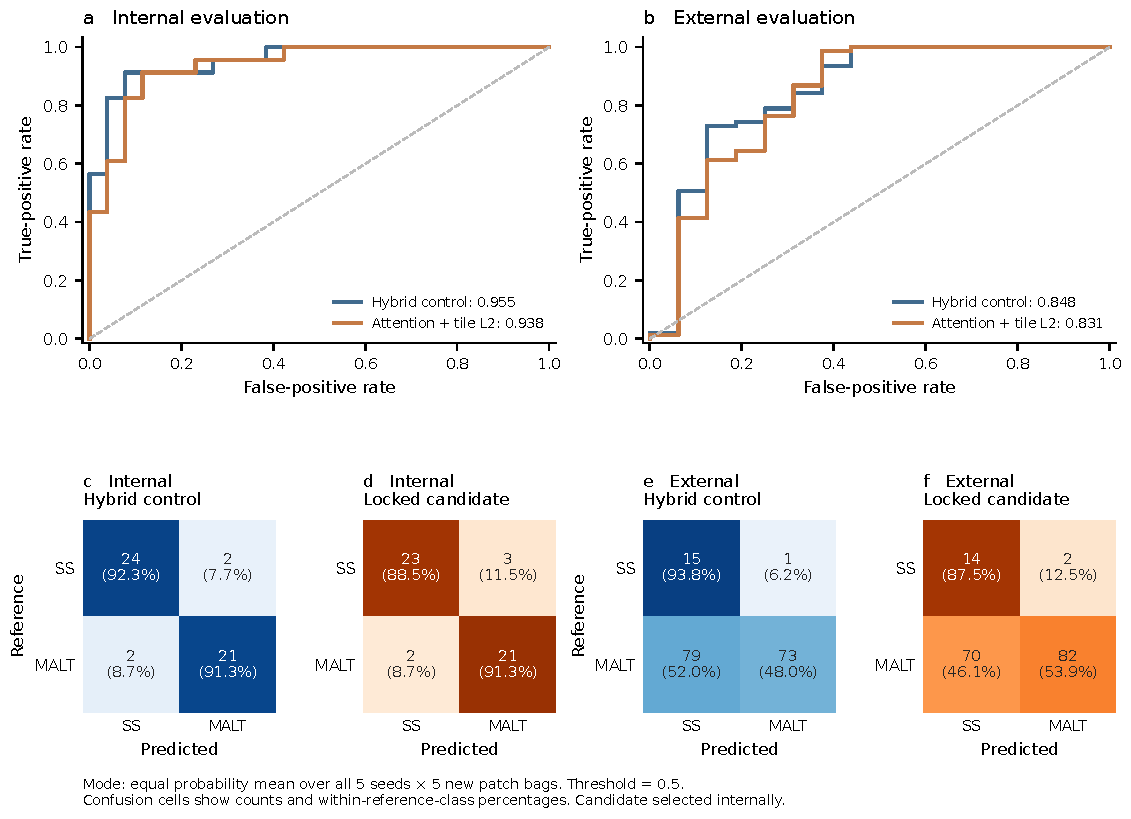
\includegraphics[width=\textwidth,height=.73\textheight,keepaspectratio]{figures/Figure_A3_locked_ensemble_ROC_confusion.pdf}
\caption{\textbf{Five-seed, five-bag probability ensembles.} All 25 probabilities per slide were averaged for each model before calculating ROC and threshold metrics. Confusion matrices use threshold 0.5 and display counts with within-reference-class percentages. These are supplementary development ensembles, not replacements for the retained primary checkpoint.}
\end{figure}
\begin{figure}[p]\centering
\fbox{\begin{minipage}[c][35mm][c]{.88\textwidth}\centering
\textbf{Omitted from this public repository copy}\\[6pt]
This figure contains tissue images or individual-slide observations.\\
The complete figure is retained in the local manuscript archive.
\end{minipage}}
\caption{\textbf{Archived model-region displays for pathological review.} Four cases represent the four threshold outcomes. Performance and visualization bags differed; paired scores for all 12 cases are in Table~S9. Colors represent within-slide-normalized latent-bank margins, not verified MALT/SS labels. The eight displayed crops retain their source pixels, with 50-$\mu$m bars. The false-negative case has unresolved legacy overlay geometry and a low-mask-coverage window, detailed in Supplementary Methods. These displays are retained as review material; they do not establish disease localization or explain errors.}
\end{figure}
\begin{figure}[p]\centering
\fbox{\begin{minipage}[c][35mm][c]{.88\textwidth}\centering
\textbf{Omitted from this public repository copy}\\[6pt]
This figure contains tissue images or individual-slide observations.\\
The complete figure is retained in the local manuscript archive.
\end{minipage}}
\caption{\textbf{Supplied histological context images.} These illustrative MALT and SS images are distinct from the model-selected regions and were not used as regional ground truth. Original pixels are unchanged. Specimen linkage, physical calibration and final descriptions remain completion item H06; no new physical scale is inferred.}
\end{figure}

\clearpage
\begingroup\small\setlength{\bibsep}{3pt}
\bibliographystyle{unsrtnat}\bibliography{references}
\endgroup
\end{document}
